%% Преамбула TeX-файла

% 1. Стиль и язык
\documentclass[utf8x]{G7-32} % Стиль (по умолчанию будет 14pt)
\usepackage[T2A]{fontenc}
\usepackage[russian]{babel}
% Остальные стандартные настройки убраны в preamble.inc.tex.
\sloppy

% Настройки стиля ГОСТ 7-32
% Для начала определяем, хотим мы или нет, чтобы рисунки и таблицы нумеровались в пределах раздела, или нам нужна сквозная нумерация.
\EqInChapter % формулы будут нумероваться в пределах раздела
\TableInChapter % таблицы будут нумероваться в пределах раздела
\PicInChapter % рисунки будут нумероваться в пределах раздела

% Добавляем гипертекстовое оглавление в PDF
\usepackage[
bookmarks=true, colorlinks=true, unicode=true,
urlcolor=black,linkcolor=black, anchorcolor=black,
citecolor=black, menucolor=black, filecolor=black,
]{hyperref}

% Изменение начертания шрифта --- после чего выглядит таймсоподобно.
% apt-get install scalable-cyrfonts-tex

\IfFileExists{cyrtimes.sty}
    {
        \usepackage{cyrtimespatched}
    }
    {
        % А если Times нету, то будет CM...
    }

\usepackage{graphicx}   % Пакет для включения рисунков

% С такими оно полями оно работает по-умолчанию:
% \RequirePackage[left=20mm,right=10mm,top=20mm,bottom=20mm,headsep=0pt]{geometry}
% Если вас тошнит от поля в 10мм --- увеличивайте до 20-ти, ну и про переплёт не забывайте:
\geometry{right=20mm}
\geometry{left=30mm}


% Пакет Tikz
\usepackage{tikz}
\usetikzlibrary{arrows,positioning,shadows}

% Произвольная нумерация списков.
\usepackage{enumerate}

% ячейки в несколько строчек
\usepackage{multirow}

% itemize внутри tabular
\usepackage{paralist,array}


% Настройки листингов.
% 8 Листинги

\usepackage{listings}

% Значения по умолчанию
\lstset{
  basicstyle= \footnotesize,
  breakatwhitespace=true,% разрыв строк только на whitespacce
  breaklines=true,       % переносить длинные строки
%   captionpos=b,          % подписи снизу -- вроде не надо
  inputencoding=koi8-r,
  numbers=left,          % нумерация слева
  numberstyle=\footnotesize,
  showspaces=false,      % показывать пробелы подчеркиваниями -- идиотизм 70-х годов
  showstringspaces=false,
  showtabs=false,        % и табы тоже
  stepnumber=1,
  tabsize=4,              % кому нужны табы по 8 символов?
  frame=single
}

% Стиль для псевдокода: строчки обычно короткие, поэтому размер шрифта побольше
\lstdefinestyle{pseudocode}{
  basicstyle=\small,
  keywordstyle=\color{black}\bfseries\underbar,
  language=Pseudocode,
  numberstyle=\footnotesize,
  commentstyle=\footnotesize\it
}

% Стиль для обычного кода: маленький шрифт
\lstdefinestyle{realcode}{
  basicstyle=\scriptsize,
  numberstyle=\footnotesize
}

% Стиль для коротких кусков обычного кода: средний шрифт
\lstdefinestyle{simplecode}{
  basicstyle=\footnotesize,
  numberstyle=\footnotesize
}

% Стиль для BNF
\lstdefinestyle{grammar}{
  basicstyle=\footnotesize,
  numberstyle=\footnotesize,
  stringstyle=\bfseries\ttfamily,
  language=BNF
}

% Определим свой язык для написания псевдокодов на основе Python
\lstdefinelanguage[]{Pseudocode}[]{Python}{
  morekeywords={each,empty,wait,do},% ключевые слова добавлять сюда
  morecomment=[s]{\{}{\}},% комменты {а-ля Pascal} смотрятся нагляднее
  literate=% а сюда добавлять операторы, которые хотите отображать как мат. символы
    {->}{\ensuremath{$\rightarrow$}~}2%
    {<-}{\ensuremath{$\leftarrow$}~}2%
    {:=}{\ensuremath{$\leftarrow$}~}2%
    {<--}{\ensuremath{$\Longleftarrow$}~}2%
}[keywords,comments]

% Свой язык для задания грамматик в BNF
\lstdefinelanguage[]{BNF}[]{}{
  morekeywords={},
  morecomment=[s]{@}{@},
  morestring=[b]",%
  literate=%
    {->}{\ensuremath{$\rightarrow$}~}2%
    {*}{\ensuremath{$^*$}~}2%
    {+}{\ensuremath{$^+$}~}2%
    {|}{\ensuremath{$|$}~}2%
}[keywords,comments,strings]

% Подписи к листингам на русском языке.
\renewcommand\lstlistingname{\cyr\CYRL\cyri\cyrs\cyrt\cyri\cyrn\cyrg}
\renewcommand\lstlistlistingname{\cyr\CYRL\cyri\cyrs\cyrt\cyri\cyrn\cyrg\cyri}


% Полезные макросы листингов.
% Любимые команды
\newcommand{\Code}[1]{\textbf{#1}}


\begin{document}

\frontmatter % выключает нумерацию ВСЕГО; здесь начинаются ненумерованные главы: реферат, введение, глоссарий, сокращения и прочее.
% НАЧАЛО ТИТУЛЬНОГО ЛИСТА
\begin{center}
\hfill \break
\small{\textbf{{МИНОБРНАУКИ РОССИИ}}}\\
\small{\textbf{{САНКТ-ПЕТЕРБУРГСКИЙ ГОСУДАРСТВЕННЫЙ}}}\\
\small{\textbf{{ЭЛЕКТРОТЕХНИЧЕСКИЙ УНИВЕРСИТЕТ}}}\\
\small{\textbf{«ЛЭТИ» ИМ. В.И. УЛЬЯНОВА (ЛЕНИНА)}}\\
\hfill \break
\normalsize{\textbf{Кафедра РС}}\\
\hfill\break
\hfill \break
\hfill \break
\hfill \break
\small{\textbf{{Курсовая работа}}}\\
\normalsize{\textbf{по дисциплине «Радиолокационные и радионавигационные системы»}}\\
\normalsize{\textbf{ТЕМА: ОБЪЕДИНЕНИЕ ИНФОРМАЦИИ В МНОГОПОЗИЦИОННЫХ
РАДИОЛОКАЦИОННЫХ КОМПЛЕКСАХ
}}\\
\hfill \break
\hfill \break
\hfill \break
\hfill \break
\hfill \break
\hfill \break
\end{center}
 
\hfill \break
 
\normalsize{ 
\begin{tabular}{cccc}
Студент гр. 8102 & \underline{\hspace{3cm}} & &Фернандес К.А. \\\\
Преподаватель & \underline{\hspace{3cm}} & &  Михайлов В. Н.\\\\
\end{tabular}
}\\
\hfill \break
\hfill \break
\begin{center} Санкт-Петербург \\
2023 \end{center}
\thispagestyle{empty} % выключаем отображение номера для этой страницы
 
% КОНЕЦ ТИТУЛЬНОГО ЛИСТА

% Команды \breakingbeforechapters и \nonbreakingbeforechapters
% управляют разрывом страницы перед главами.
% По-умолчанию страница разрывается.

% \nobreakingbeforechapters
% \breakingbeforechapters

%% Также можно использовать \Referat, как в оригинале
\begin{abstract}
Это пример каркаса расчётно-пояснительной записки, желательный к использованию в РПЗ проекта по курсу РСОИ.

Данный опус, как и более новые версии этого документа, можно взять по адресу (\url{https://github.com/rominf/latex-g7-32}).

Текст в документе носит совершенно абстрактный характер.
\end{abstract}

%%% Local Variables: 
%%% mode: latex
%%% TeX-master: "rpz"
%%% End: 

\tableofcontents
%\Defines % Необходимые определения. Вряд ли понадобться
\begin{description}
\item[Распределённый] Слово, которое нельзя употреблять. Но надо протестировать длинные строки в глоссарии.
\end{description}

%%% Local Variables:
%%% mode: latex
%%% TeX-master: "rpz"
%%% End:

\Abbreviations %% Список обозначений и сокращений в тексте
\begin{description}
\item[РЛС] Радиолокационная станция
\item [ЛТ] Ложная тревога
\item [ВЛТ] Вероятность ложной тревоги
\item [ВПО] Вероятность правильного обнаружения
\item [ЭПР] Эффективная площадь рассеяния
\end{description}

%%% Local Variables:
%%% mode: latex
%%% TeX-master: "rpz"
%%% End:


\Introduction

Данный документ представляет собой отчет к курсовой расчетной работе по дисциплине "Радиолокационные и радионавигационные системы". 
В ходе данной работы было выполнено следующее: 
\begin{itemize}
    \item проведено ознакомление с методами объединения информации, 
    \item построена зависимость вероятности правильного обнаружения в зависимости от дальности для одной РЛС, 
    \item оценен процент площади, на которой происходит обнаружение с вероятностью 95 \% для одиночной РЛС, расположенной в центре области, 
    \item обеспечено обнаружение с вероятностями правильного обнаружения $D_0 = 95 \%$, вероятностью ложной тревоги $F_0 = 10^{-8}$ в заданной области, 
    \item для обеспечения данной конфигурации были выбраны количество и конфигурация РЛС, 
    \item  выбран критерий обнаружения в комплексе, 
    \item  построены зоны обнаружения для выбранной конфигурации РЛС без объединения, при объединении по схемам «И», «ИЛИ» и выбранному критерию обнаружения. 
\end{itemize} 

В ходе данной работы был использован вариант №24. 

\mainmatter % это включает нумерацию глав и секций в документе ниже

\chapter{Теоретические сведения}
\label{cha:impl}
Для сигнала со случайной амплитудой, распределенной по закону Релея, и 
равномерно распределенной начальной фазой вероятность правильного обнаружения: 
$$ D = F^{\frac{1}{1 + 0.5 Q^2}} $$
где D – вероятность правильного обнаружения, а F – вероятность ложной тревоги. 
Величина 
$$ Q = \sqrt{\frac{2E_{res}}{N_0}} $$
численно равная отношению сигнал-помеха по напряжению на выходе согласованного, 
называется параметром обнаружения или отношением сигнал/шум. 
Найдем сначала найдем энергию на входе приемника $E_{res}$. Для этого рассчитаем 
плотности потока энергии у цели, удаленной на расстояние $r_1$ от передающей антенны: 
$$ I_t = \frac{P_p G_{tr}(\alpha, \beta) }{4 \pi r_{1}^2} $$
где $P_p$ – импульсная мощность. $G_{tr}$ – коэффициент усиления передающей антенны. 
Реальные передающие антенны принято сравнивать с идеальной ненаправленной 
антенной. Плотность потока мощности у таких идеальных антенн на расстоянии r от центра 
антенны составит:
$$I_0 = \frac{P}{4 \pi r^2}$$
где $P$ – подводимая к антенне мощность.
Эффективная площадь приема 
и коэффициент усиления антенны взаимосвязаны: 
$$G = \frac{4 \pi A}{\lambda^2}$$

Формулу мощности принимаемого сигнала 
можно записать так: 
$$ P_{res} = \frac{P_p G_{tr} \sigma A_{res} }{(4 \pi)^2 r^4} $$

$$ E_{res} = \frac{P_p \tau_p G^2 \sigma \lambda^2 }{(4 \pi)^3 (r^2 + h^2)^2} $$
\chapter{Моделирование одиночной РЛС}
\label{cha:analysis}

В данном разделе были рассмотрены пункты, связанные с моделированием случая одиночно расположенной радиолокационной станции. На рис. \ref{fig:RLS_1_dist} представлена зависимость вероятности правильного обнаружения от дальности до объекта.

\begin{figure}
    \centering
    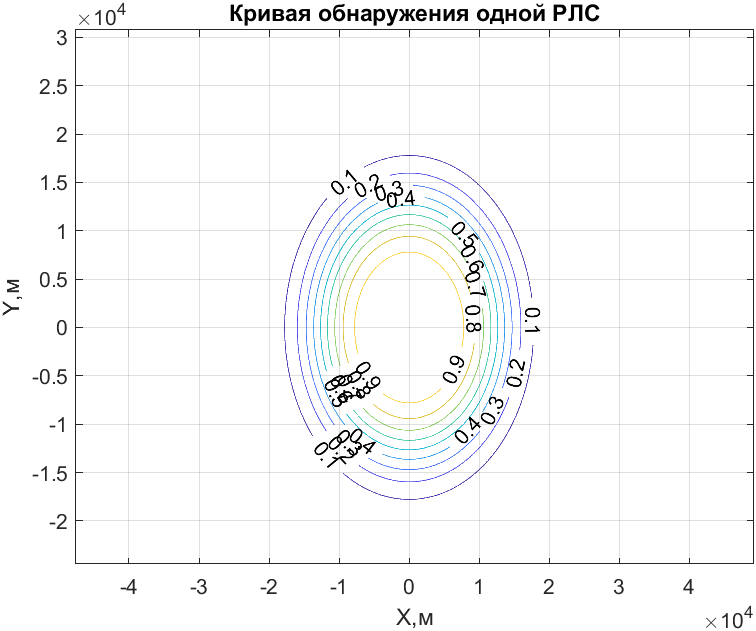
\includegraphics{figures/SingleRLS.png}
    \caption{Зависимость вероятности обнаружения от дальности для одиночно расположенной РЛС}
    \label{fig:RLS_1_dist}
\end{figure}

\chapter{Моделирование систем из нескольких РЛС}

\section{Теоретическая часть}

Объединение двух РЛС с идентичными параметрами $D$ и $F$ позволяет получить схемы объединения РЛС по различным критериям, означающими принятие решения в пользу альтернативы при данном решении для определенного количества РЛС. Данный принцип порождает две минимаксные схемы «И» и «ИЛИ». Объединение по схеме «ИЛИ» приводит к улучшению $D(D_c > D)$, но ухудшает $F(F_c > F)$, и наоборот, схема «И» ухудшает $D(D_c < D)$, но улучшает $F(F_c < F)$. В схеме объединения «И» вероятности будут определяться как $F_1 = F_2 = \sqrt{F_c} = \sqrt{F_e}$ где $F_c$ – вероятность ЛТ эквивалентной РЛС, а $F_e$ – вероятность ЛТ комплекса.
В схеме «ИЛИ» эти вероятности будут равны $F_1 = F_2 = 1 - \sqrt{1 - F_c} = 1 - \sqrt{1 - F_e}.$
В данной работе рассматривается ситуация объединения 4 и 18 РЛС. 

\section{Моделирование системы из 4 РЛС}

\begin{figure}
    \centering
    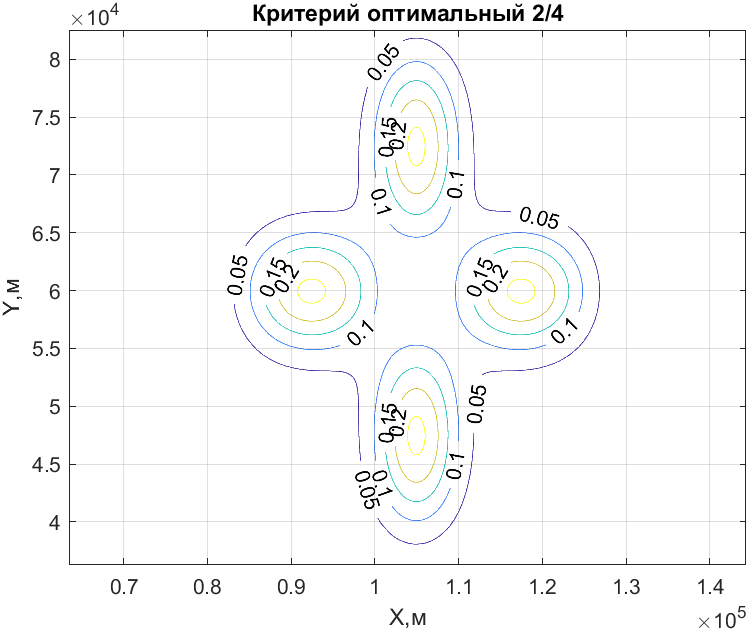
\includegraphics{figures/2_4_RLS.png}
    \caption{Критерий 2 из 4 для 4х РЛС}
    \label{fig:my_label}
\end{figure}

\begin{figure}
    \centering
    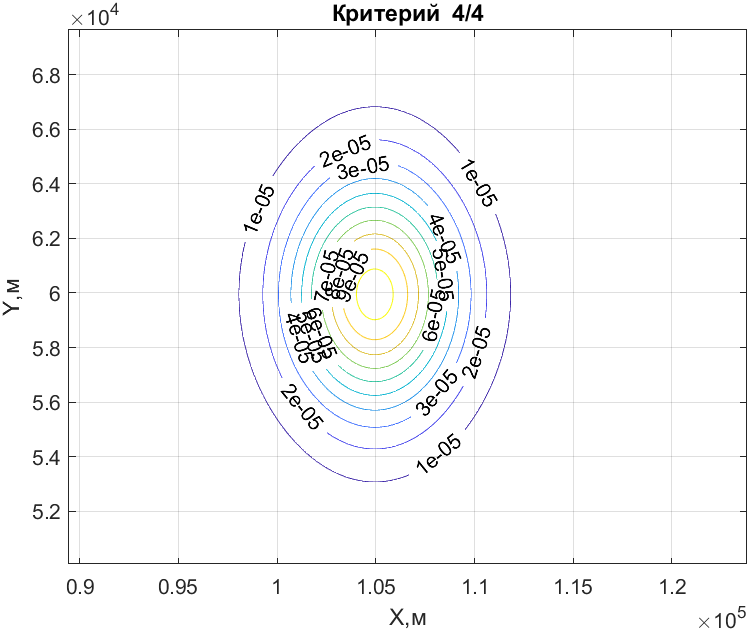
\includegraphics{figures/4_4_RLS.png}
    \caption{Критерий 4 из 4 для 4х РЛС}
    \label{fig:my_label}
\end{figure}

\begin{figure}
    \centering
    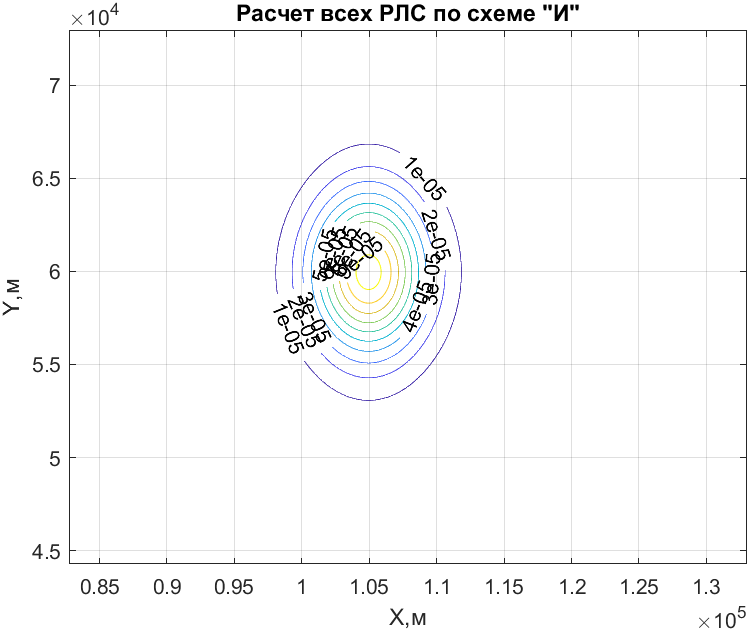
\includegraphics{figures/AND_RLS_4.png}
    \caption{Объединение для 4х РЛС по схеме "И"}
    \label{fig:my_label}
\end{figure}

\begin{figure}
    \centering
    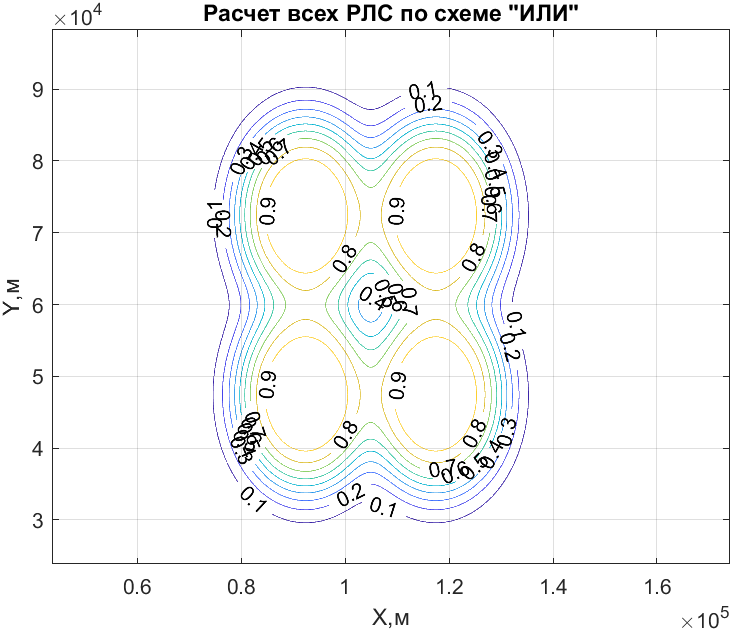
\includegraphics{figures/OR_RLS_4.png}
    \caption{Объединение для 4х РЛС по схеме "ИЛИ"}
    \label{fig:my_label}
\end{figure}

\begin{figure}
    \centering
    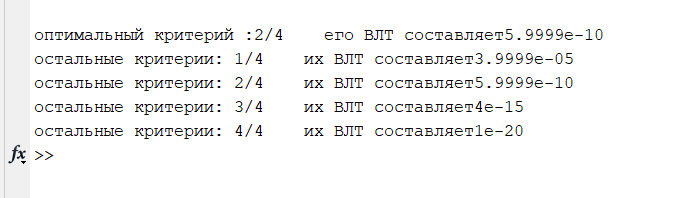
\includegraphics[scale = 0.7]{figures/VLT_4.png}
    \caption{Вероятность ложной тревоги для 4 РЛС}
    \label{fig:my_label}
\end{figure}

\section{Моделирование системы из 18 РЛС}

\begin{figure}
    \centering
    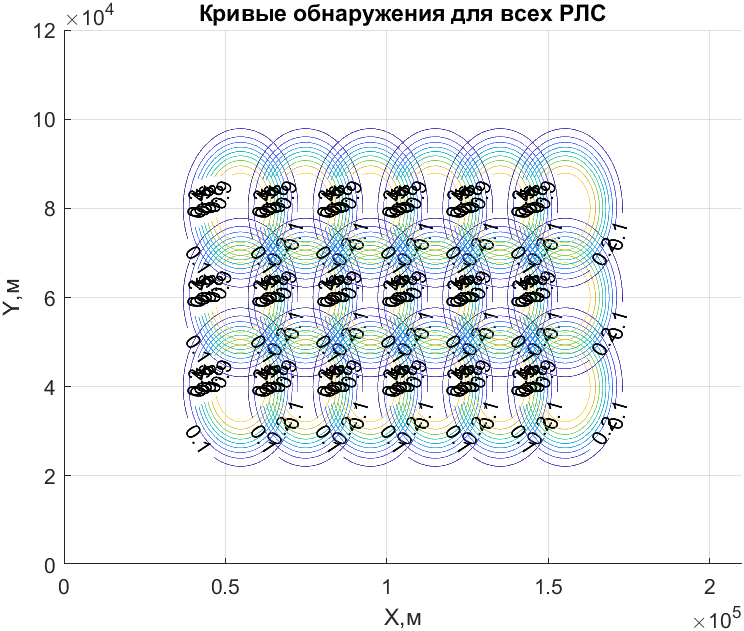
\includegraphics{figures/ALL_RLS.png}
    \caption{Кривые обнаружения для всех РЛС}
    \label{fig:my_label}
\end{figure}

\begin{figure}
    \centering
    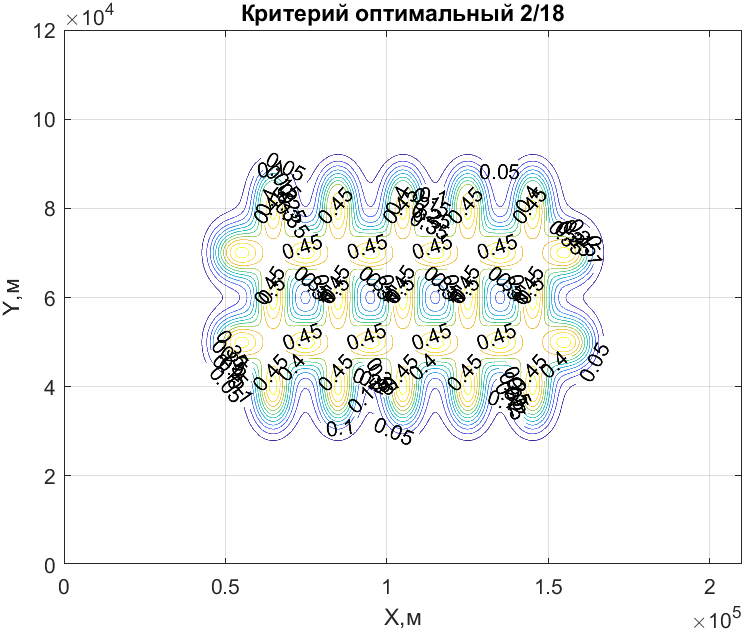
\includegraphics{figures/2_18_RLS.png}
    \caption{Оптимальный критерий обнаружения для 18 РЛС}
    \label{fig:my_label}
\end{figure}

\begin{figure}
    \centering
    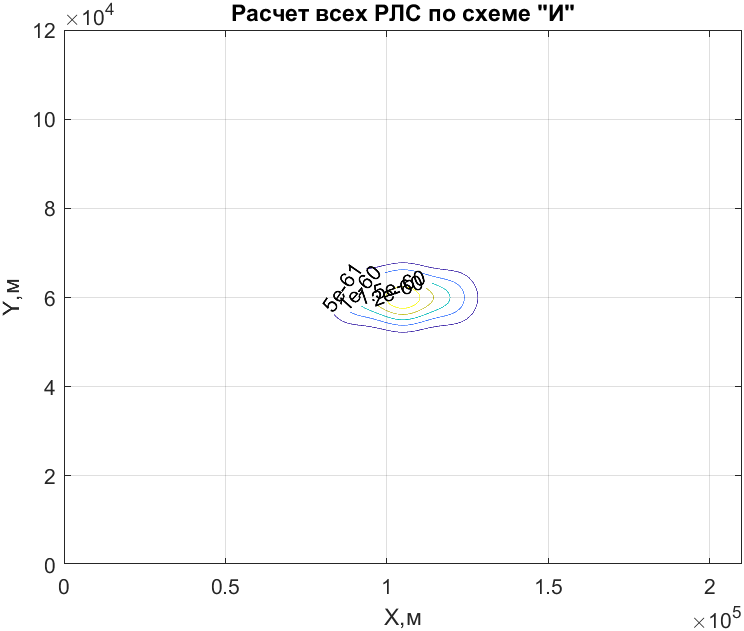
\includegraphics{figures/AND_RLS_18.png}
    \caption{Объединение всех РЛС по схеме "И"}
    \label{fig:my_label}
\end{figure}

\begin{figure}
    \centering
    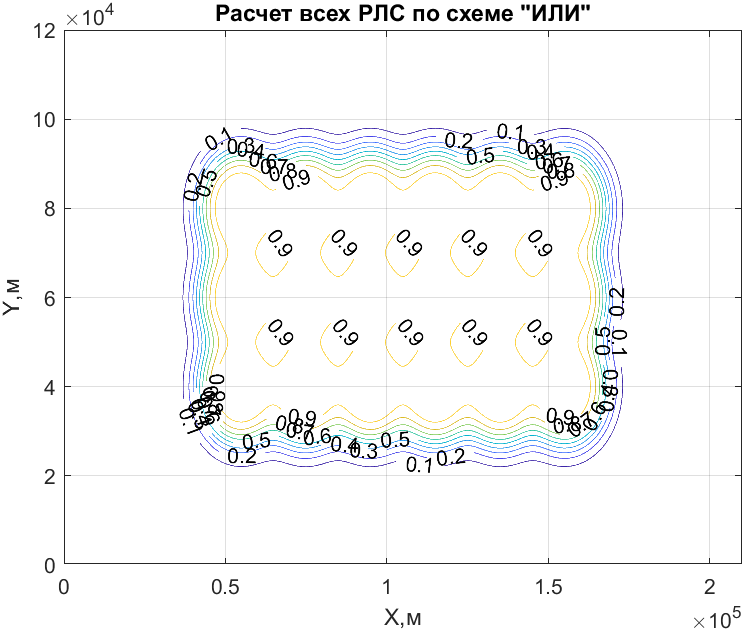
\includegraphics{figures/OR_RLS_18.png}
    \caption{Объединение всех РЛС по схеме "ИЛИ"}
    \label{fig:my_label}
\end{figure}

\begin{figure}
    \centering
    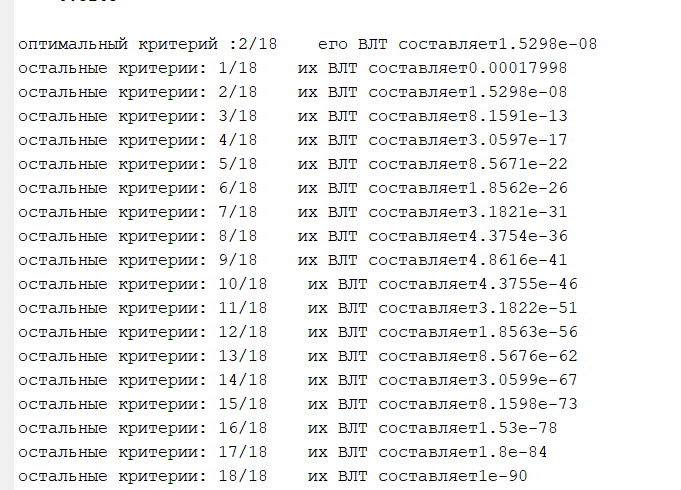
\includegraphics[scale = 0.7]{figures/VLT_18.png}
    \caption{Вероятность ложной тревоги для 18 РЛС}
    \label{fig:my_label}
\end{figure}

\include{40-impl}
%\chapter{Экспериментальный раздел}
\label{cha:research}

В данном разделе проводятся вычислительные эксперименты.
А на рис.~\ref{fig:spire01} показана схема мыслительного процесса автора...

\begin{figure}
  \centering
  \includegraphics[width=\textwidth]{figures/pic01}
  \caption{Как страшно жить}
  \label{fig:spire01}
\end{figure}


%%% Local Variables:
%%% mode: latex
%%% TeX-master: "rpz"
%%% End:


\backmatter %% Здесь заканчивается нумерованная часть документа и начинаются ссылки и
            %% заключение

\Conclusion % заключение к отчёту

В процессе разработки системы обнаружения целей, важным этапом является выбор оптимальной схемы объединения данных от нескольких РЛС. Она должна обеспечивать максимальную вероятность истинного обнаружения цели при заданной вероятности ложного обнаружения. 

Увеличение числа обнаружений не менее M из N приводит к уменьшению вероятности ложной тревоги и увеличению вероятности пропуска цели. Однако, выбор конкретной схемы объединения может повлиять на эти вероятности. Например, схема «ИЛИ» обеспечивает большую зону видимости, но имеет проблемы с вероятностью ложной тревоги. С другой стороны, схема «И» имеет низкую вероятность правильного обнаружения, что приводит к уменьшению зоны видимости.

В случае использования схемы «ИЛИ», увеличение числа РЛС может привести к увеличению зоны видимости системы. Однако, при этом может возникнуть проблема с вероятностью ложной тревоги. В то же время, использование схемы «И» может привести к катастрофически низкой вероятности правильного обнаружения цели, что снижает зону видимости. 

Таким образом, выбор оптимальной схемы объединения данных является важным шагом в разработке системы обнаружения целей. При этом необходимо учитывать как требования по вероятности истинного обнаружения и ложного обнаружения, так и возможные проблемы с зоной видимости при использовании конкретной схемы.


\bibliographystyle{gost780u}
%\bibliography{rpz}

\begin{thebibliography}{3}
\bibitem{RM}
Гришин Ю. П., В. П. Ипатов Радиотехнические системы / Высшая школа, Москва. 1990 --- 496 с.

\bibitem{PPK}
Под ред Сколника М. И. Справочник по радиолокации, Книга 1 / Техносфера, Москва. 2015 --- 672 с.

\bibitem{PPK}
Под ред Сколника М. И. Справочник по радиолокации, Книга 2 / Техносфера, Москва. 2015 --- 680 с.

\bibitem{PPK}
Левин Б. Р. Статистическая радиотехника / Советское радио, Москва. 1969--- 752 с.

\appendix   % Тут идут приложения

\chapter{Задание на курсовую расчетную работу}
\label{cha:appendix1}

Тема работы: Объединение информации в многопозиционных радиолокационных комплексах. \\

Используемый вариант: 24. 

\begin{table}[]
\begin{tabular}{llllllllllll}
\hline
\multicolumn{1}{|l|}{$P_p$} & \multicolumn{1}{l|}{$\tau_p$} & \multicolumn{1}{l|}{$G$}   & \multicolumn{1}{l|}{$k_n$}  & \multicolumn{1}{l|}{$T_a$} & \multicolumn{1}{l|}{АЧХ}         & \multicolumn{1}{l|}{f, mHz} & \multicolumn{1}{l|}{$\sigma, m^2$} & \multicolumn{1}{l|}{$V_m$} & \multicolumn{1}{l|}{X,км} & \multicolumn{1}{l|}{Y,км} & \multicolumn{1}{l|}{$F_{rls}*10^{-5}$} \\ \hline
\multicolumn{1}{|l|}{3.5}     & \multicolumn{1}{l|}{3}       & \multicolumn{1}{l|}{400} & \multicolumn{1}{l|}{2,4} & \multicolumn{1}{l|}{24} & \multicolumn{1}{l|}{Кол.} & \multicolumn{1}{l|}{170}    & \multicolumn{1}{l|}{10}    & \multicolumn{1}{l|}{300}     & \multicolumn{1}{l|}{210}   & \multicolumn{1}{l|}{120}   & \multicolumn{1}{l|}{1}         \\ \hline
                              &                              &                          &                          &                         &                                  &                             &                            &                              &                            &                            &                                \\
                              &                              &                          &                          &                         &                                  &                             &                            &                              &                            &                            &                               
\end{tabular}
\end{table}
%\chapter{Еще картинки}
\label{cha:appendix2}

\begin{figure}
\centering
\caption{Еще одна картинка, ничем не лучше предыдущей. Но надо же как-то заполнить место.}
\end{figure}

%%% Local Variables: 
%%% mode: latex
%%% TeX-master: "rpz"
%%% End: 


\end{document}

%%% Local Variables:
%%% mode: latex
%%% TeX-master: t
%%% End:
